\documentclass{notes}

\usepackage{hyperref}
\usepackage{amssymb}
\usepackage[
    backend=biber,
    sorting=none,
    style=numeric-comp,
    citestyle=numeric-comp,
    url=false,
    doi=true
]{biblatex}
\usepackage{siunitx}
\usepackage{tcolorbox}

\addbibresource{ref.bib}

\title{Tokamak startup model in DREAM}
\author{Mathias Hoppe}

\newcommand{\tDREAM}{{\mdseries\DREAM}}
\newcommand{\tDYON}{{\mdseries\DYON}}

\newcommand{\ee}{\mathrm{e}}

\newcommand{\IMK}{I_{\rm MK2}}
\newcommand{\Ip}{I_{\rm p}}
\newcommand{\Iw}{I_{\rm wall}}
\newcommand{\Vl}{V_{\rm loop}}
\newcommand{\Vle}{\Vl^{({\rm edge})}}
\newcommand{\Vlw}{\Vl^{({\rm wall})}}
\newcommand{\Rp}{R_{\rm p}}
\newcommand{\Vp}{V_{\rm p}}

\newcommand{\psie}{\psi_{\rm edge}}
\newcommand{\psiw}{\psi_{\rm wall}}

%\newcommand{\summarytitle}[1]{{\bf\large Summary --- #1}}
\newtcolorbox{summarybox}[1]{colback=red!5!white, colframe=red!75!black, fonttitle=\bfseries, title=Summary --- #1}
\newtcolorbox{taskbox}[1]{colback=green!5!white, colframe=green!55!black, fonttitle=\bfseries, title=Tasks --- #1}

\begin{document}
    \maketitle

    In this document we review the requirements for \DREAM\ to function as a
    basic tokamak start-up code, similar to \DYON~\cite{Kim2012}. The code
    \DYON\ seems in turn to have been inspired by previous work, such
    as~\cite{Lloyd1996}.

    Although \DREAM\ provides the ability to simulate a spatially homogeneous
    (1D) plasma, the model used in \DYON\ is 0D and does not admit a
    straightforward generalization to 1D. Hence, we will here assume that
    \DREAM\ is run in 0D mode and focus on which models are currently missing
    from the code.

    \tableofcontents

    \section{Circuit equation for plasma current}
    \DYON\ uses a two-ring model for the the plasma current. In addition to the
    plasma ring, a significant eddy current is expected to be induced in the
    so-called MK2 ring (a divertor mechanical support structure), which has the
    lowest electrical resistance of the various vessel components. The model in
    \DYON\ therefore is
    \begin{subequations}\label{eq:dyonV}
        \begin{align}
            \Vl &= \Ip\Rp + L_{\rm p}\frac{\dd\Ip}{\dd t} + M\frac{\dd\IMK}{\dd t},\label{eq:dyonVp}\\
            \Vl &= \IMK R_{\rm MK2} + L_{\rm MK2}\frac{\dd\IMK}{\dd t} + M\frac{\dd\Ip}{\dd t},\label{eq:VloopMK2}
        \end{align}
    \end{subequations}
    where $\Vl$ is the loop voltage, $\Rp$ the plasma resistance, $M$ the
    mutual inductance and the self-inductance
    \begin{equation}
        L_{\rm p} = \mu_0 R\left( \ln\frac{8R}{a} + \frac{l_i}{2} - 2 \right),
    \end{equation}
    with internal inductance
    \begin{equation}
        l_i = \frac{2\int_0^a B_\theta^2 r\,\dd r}{a^2 B_{\theta a}^2}.
    \end{equation}
    The self-inductance $L_{\rm MK2}$ of the MK2 ring is not specified.

    \subsection{Current formulation}
    The current model in \DREAM\ consists of the following equations:
    \begin{subequations}
        \begin{align}
            2\pi\mu_0\left\langle\bb{B}\cdot\nabla\phi\right\rangle
            \frac{j_{\rm tot}}{B} &= \frac{1}{V'}\frac{\partial}{\partial r}\left[
                V'\left\langle\frac{\left|\nabla r\right|^2}{R^2}\right\rangle
                \frac{\partial\psi}{\partial r}
            \right],\label{eq:currdiff}\\
            %
            \psie &= \psiw - M_{\rm ew} \Ip,\label{eq:psie}\\
            \psiw &= -L_{\rm ext}\left(\Ip + \Iw\right),\label{eq:psiw}\\
            \Vl &= \Rp\Ip,\label{eq:RpIp}\\
            \Vlw &= R_{\rm wall}\Iw,\label{eq:RwIw}\\
            \frac{\partial\psi}{\partial t} &= \Vl,
        \end{align}
    \end{subequations}
    We begin by showing that this model yields equations~\eqref{eq:dyonV}, with
    $\Vl=0$. To do so, we first note that the time derivative of the current
    diffusion equation~\eqref{eq:currdiff} can be regarded as an equation for
    the voltage difference $\Delta V$ between $\Vle$ and $\Vl$ inside the
    plasma:
    \begin{equation}
        \Delta V = \Vle-\Vl = L\frac{\dd\Ip}{\dd t}.
    \end{equation}
    (for a derivation of this, see Appendix~\ref{app:induction}).
    The edge loop voltage can be expressed in terms of the loop voltage on the
    wall using~\eqref{eq:psie}, which can in turn be substituted
    for~\eqref{eq:psiw}:
    \begin{equation}
        \begin{gathered}
            \Vlw-M_{\rm ew}\frac{\dd\Ip}{\dd t} = \Rp\Ip + L\frac{\dd\Ip}{\dd t},\\
            \Longleftrightarrow\\
            -L_{\rm ext}\left(\frac{\dd\Ip}{\dd t} + \frac{\dd I_{\rm wall}}{\dd t}\right)
            -M_{\rm ew}\frac{\dd\Ip}{\dd t} = \Rp\Ip + L\frac{\dd\Ip}{\dd t}.
        \end{gathered}
    \end{equation}
    Collecting terms, we arrive at
    \begin{equation}\label{eq:circ1}
        \Rp\Ip + \left(L + L_{\rm ext} + M_{\rm ew}\right)\frac{\dd\Ip}{\dd t}
        + L_{\rm ext}\frac{\dd I_{\rm wall}}{\dd t} = 0,
    \end{equation}
    which, although not identical to~\eqref{eq:dyonVp}, has the same structure,
    with $\Vl=0$. Similarly, we can combine~\eqref{eq:psiw} and~\eqref{eq:RwIw}
    to obtain
    \begin{equation}\label{eq:circ2}
        R_{\rm wall}I_{\rm wall} + L_{\rm ext}\left(\frac{\dd I_{\rm wall}}{\dd t} + \frac{\dd\Ip}{\dd t} \right) = 0,
    \end{equation}
    which has the same structure as~\eqref{eq:VloopMK2}.

    \subsection{Required modifications}
    Based on the derivation of the \DYON\ equations above, one could notice that
    only equation~\eqref{eq:psiw} appears in the derivation of both circuit
    equations. By modifying this term appropriately, we could therefore cause a
    prescribed loop voltage to appear in both circuit equations~\eqref{eq:circ1}
    and~\eqref{eq:circ2}. But how do we justify such a term?

    As a matter of fact, equation~\eqref{eq:psiw} should actually be written
    \begin{equation}
        \psiw = \psi_{\rm sym} - L_{\rm ext}\left( \Ip + \Iw \right),
    \end{equation}
    where $\psi_{\rm sym}$ is the poloidal flux at the symmetry axis, $R=0$.
    Since the poloidal flux is typically defined as the integral
    \begin{equation}
        \psi(r) = \int_0^{R(r)} \bb{B}\cdot\zhat\,\dd R,
    \end{equation}
    $\psi_{\rm sym}=\psi(R=0)$ is usually taken to as zero. The poloidal flux
    can however be defined with an offset $\psi_0$, and this offset can have
    a time dependence. We can therefore include this term explicitly in
    equation~\eqref{eq:psiw} and evolve it according to a prescribed loop
    voltage:
    \begin{equation}
        \psi_{\rm sym} = \Vl^{(\rm appl)}.
    \end{equation}
    Physically, we can think of this as a transformer passing through $R=0$
    applying a loop voltage $\Vl^{(\rm appl)}$.

    As for the MK2 structure, we can use the regular ``self-consistent''
    poloidal flux boundary conditions and simply think of ``wall'' as ``MK2''.
    The wall radius must then be chosen in order to obtain the appropriate
    inductance.

    With these modifications, the corresponding circuit equations in \DREAM\
    are
    \begin{equation}
        \begin{aligned}
            V_{\rm loop} &= R_{\rm p}\Ip + \left( L + L_{\rm ext} + M_{\rm ew} \right)\frac{\dd\Ip}{\dd t} + L_{\rm ext}\frac{\dd\Iw}{\dd t},\\
            V_{\rm loop} &= R_{\rm wall}\Iw + L_{\rm ext}\frac{\dd\Iw}{\dd t} + L_{\rm ext}\frac{\dd\Ip}{\dd t}
        \end{aligned}
    \end{equation}

    \begin{summarybox}{Loop voltage}
        %
        In summary, an applied loop voltage would require the following
        modifications to \DREAM:
        \begin{enumerate}
            \item Add an unknown $\psi_{\rm sym}$, representing the poloidal flux
            at the symmetry axis.
            %
            \item Add $\psi_{\rm sym}$ to the RHS of equation~\eqref{eq:psiw}.
            %
            \item Add the equation
            $\partial\psi_{\rm sym}/\partial t = \Vl^{(\rm appl)}$ to the system
            of equations.
        \end{enumerate}
    \end{summarybox}

    \section{Neutral particles}
    Before we get into the details of the energy and particle balance equations,
    we should note the special treatment granted to neutral particles in \DYON.
    In the code, it is imagined that the central part of the plasma volume is
    fully ionized and screens out neutral particles. As such, the plasma
    consists mutliple overlapping volumes (also illustrated i
    figure~\ref{fig:volumes}):
    \begin{itemize}
        \item {\bf Plasma volume $\Vp$:} This is the typical plasma volume in
        \DREAM.
        %
        \item {\bf Neutral volume for species $i$, $V_{n,i}$:} This volume is
        equal to $\Vp$, minus the volume of the plasma which is fully ionized.
        %
        \item {\bf Tokamak volume $V$:} This volume typically is not used in
        \DREAM. For the sake of this startup model, it could be provided as an
        input parameter.
    \end{itemize}
    Based on these definitions, we always have $V_{n,i}\leq \Vp < V$.

    \begin{figure}
        \centering
        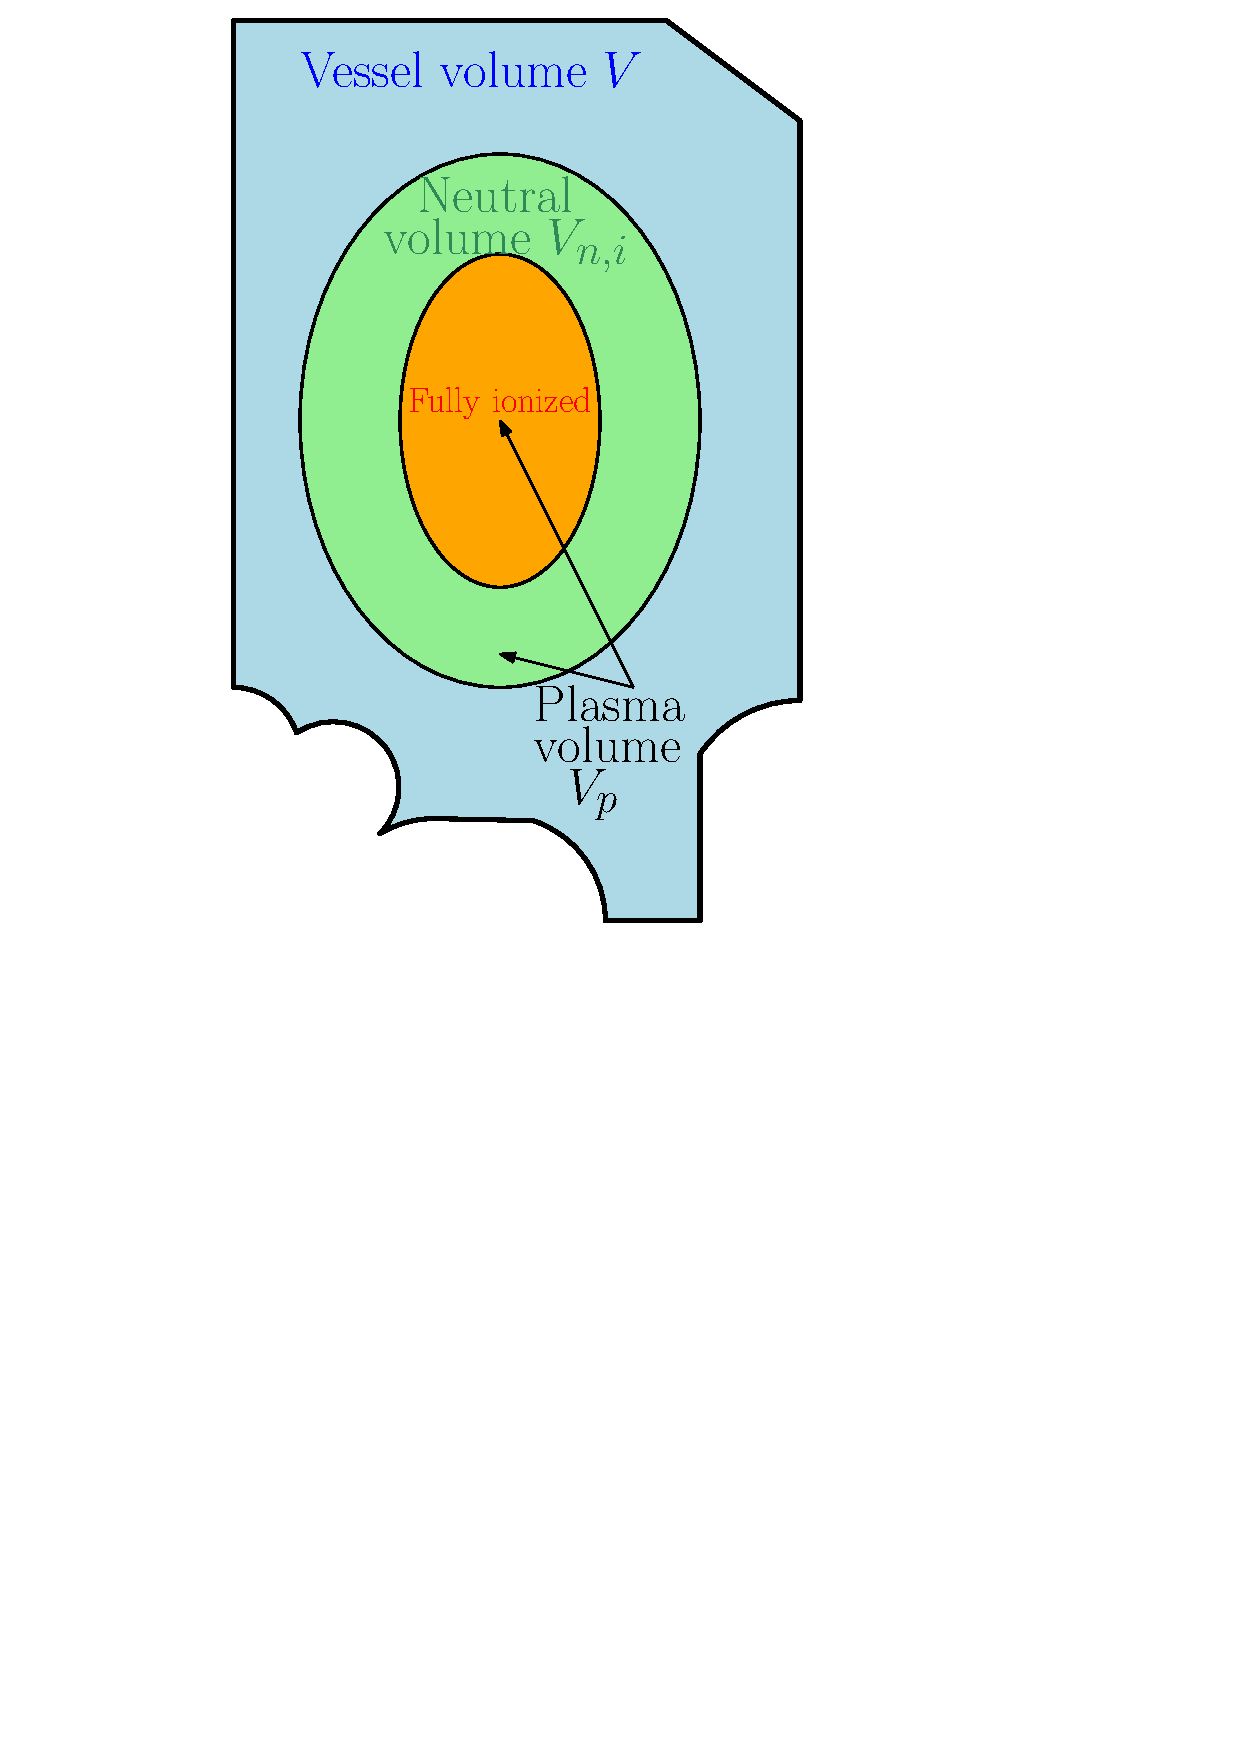
\includegraphics[width=0.4\textwidth]{figs/startup_volume.pdf}
        \caption{Illustration of how the various volumes are defined in \DYON.
        The vacuum vessel volume is denoted $V$ and is the combination of the
        blue, green and orange regions. The plasma volume $\Vp$ consists of both
        the neutral (green) and fully ionized (orange) regions, while the
        neutral volume for ion species $i$, denoted $V_{n,i}$, is just the green
        region.
        }
        \label{fig:volumes}
    \end{figure}

    The neutral volume enters in many terms of the particle and energy balance
    equations through a factor which we call $\alpha_i = V_{n,i}/\Vp$, i.e.\
    the ratio of neutral to plasma volume for species $i$. In addition to this
    factor, the neutral volume coefficient
    \begin{equation}
        \gamma_{n,i} = 1 - \frac{\Vp-V_{n,i}}{V},
    \end{equation}
    also appears in a few places. In particular, we note that $\gamma_{n,i}V$ is
    the total neutral volume, i.e.\ the volume occupied by neutrals, including
    inside the plasma (except for the fully ionized volume).

    The neutral volume is expressed in terms of the mean free path $\lambda_i$
    of neutrals of species $i$:
    \begin{equation}
        V_{n,i} = \begin{cases}
            2\pi R\left[ \pi\kappa a^2 - \pi\kappa\left( a - \lambda_i \right)^2\right], &\quad\text{if }\lambda_i\leq a,\\
            \Vp, &\quad\text{if }\lambda_i > a.
        \end{cases}
    \end{equation}
    \DYON\ uses elliptical flux surfaces with elongation $\kappa$. In \DREAM,
    however, we also allow for a finite triangularity $\delta$ which we could
    try to account for. 

    While $\lambda_i$ is not given in the \DYON\ paper~\cite{Kim2012}, it is
    given in Ref.~\cite{Lloyd1996} as
    \begin{equation}
        \lambda_i = \frac{v_i}{n_e I_i^{(0)}},
    \end{equation}
    where the ionization rate for species $i$ is $I_i^{(0)}=I_i^{(0)}(n_e,T_e)$
    and $v_i = \sqrt{2T_i/m}$. (In~\cite{Lloyd1996} they actually only specify
    $\lambda_i$ for deuterium, but I think it should generalize like this to
    arbitrary ion species)

    \section{Energy balance}\label{sec:energy}
    \DYON\ considers the energy of both electrons and the various ion species
    present in the plasma. The equations used for the energy balance are mostly
    similar to those in \DREAM, with some deviations.

    \subsection{\tDYON\ electron equations}
    The model in \DYON\ consists of the following equations:
    \begin{equation}
        \frac{\dd W_e}{\dd t} = P_{\Omega} - \left(P_{\rm ioniz} + P_{\rm rad}\right)
        - P_{\rm equi} - P_{\rm conv}^e,
    \end{equation}
    where
    \begin{align}
        P_{\Omega} &= \frac{\Ip^2\Rp}{\Vp}, \tag{Ohmic heating}\\
        %
        P_{\rm ioniz} + P_{\rm rad} &= \sum_i\left\{
            \frac{V_{n,i}}{\Vp}\left[ L_{\rm line} + \Delta W_i^{(0)} I_i^{(0)} \right]+\right.\nonumber\\
            &+ \left.
            \sum_{j\geq 1} \left[
                L_{\rm line} + L_{\rm free} + \Delta W_i^{(j)}\left( I_i^{(j)} - R_i^{(j)} \right)
            \right]
        \right\}, \tag{Ionization \& radiation}\\
        %
        P_{\rm equi} &= \mathrm{const}\times n_e\ln\Lambda\frac{T_e-T_i}{T_e^{3/2}}\sum_{ij}
            \frac{n_i^{(j)}\left(Z_i^{(j)}\right)^2}{m_i}, \tag{Electron-ion collisions}\\
        %
        P_{\rm conv}^e &= \frac{1}{\tau_e}W_e,\tag{Convective transport}
    \end{align}
    We first note that although written slightly differently, the ohmic heating
    and equilibration terms $P_\Omega$ and $P_{\rm equi}$ are identical to those
    appearing in \DREAM. Convective transport can also be modelled in \DREAM,
    and the only complication arising from $P_{\rm conv}^e$ is the determination
    of the electron confinement time $\tau_e$ (taken equal to the deuterium
    confinement time) which will be discussed in section~\ref{sec:confinement}.
    The only term looking somewhat different from what we have in \DREAM\ is the
    ionization and radiation loss term, $P_{\rm ioniz}+P_{\rm rad}$, which
    differs by a factor $V_{n,i}/\Vp$ on the neutral loss term. This is due to
    the neutral screening effect which is modelled in \DYON\ (but currently not
    in \DREAM), and should be taken into account.

    \subsection{\tDYON\ ion equations}
    The ion energy balance equation for species $i$ in \DYON\ takes the form
    \begin{equation}
        \frac{\dd W_{\rm ions}}{\dd t} = P_{\rm equi} - P_{\rm CX} - P_{\rm conv}^{\rm ions},
    \end{equation}
    where $P_{\rm equi}$ is the same as in the electron energy balance equation
    and
    \begin{align}
        P_{\rm CX} &= \frac{V_{n,D}}{\Vp}\left[
            \frac{3}{2}n_D^{(0)}\left(T_{\rm ions}-T_0\right)\sum_i R_{i,{\rm cx}}^{(1)}n_i^{(1)}
        \right], \tag{Charge exchange}\\
        %
        P_{\rm conv}^{\rm ions} &= \sum_i\sum_{j\geq 1}\frac{3}{2}\frac{n_i^{(j)}T_{\rm ions}}{\tau_D}.
        \tag{Convective transport}
    \end{align}
    where $T_0 = \SI{0.026}{eV}$ corresponds to the temperature of the
    lower-energy deuterium atom in the charge exchange reaction, assumed to be
    at room temperature, and $R_{i,{\rm cx}}^{(1)}$ is the charge exchange
    recombination coefficient (the one called CCD in Open-ADAS). It is assumed
    that only deuterium is available for donating electrons in a charge exchange
    reaction, and that all ions are transported at the same rate $\tau_D$
    (although only ionized particles, with $Z_0>0$, are transported).

    Further, we note that \DYON\ assumes that all ions have the same
    temperature. In \DREAM, we only assume that the temperature is the same in
    every charge state, but allow for different ion species to have different
    temperatures.

    \subsection{Required modifications}
    Based on the discussion above, five modifications will be required in \DREAM\
    to match the energy balance model in \DYON:
    \begin{summarybox}{Energy balance}
        \begin{enumerate}
            \item Introduce the neutral volume for species $i$, $V_{n,i}$, as an
            unknown quantity and multiply the $Z_0=0$ term by the ratio of
            neutral to plasma volume in the \texttt{RadiatedPowerTerm} in \DREAM.
            %
            \item Add the particle confinement time $\tau_p$ as an unknown quantity
            that is solved for. The details of how to solve for this quantity are
            discussed in section~\ref{sec:confinement}.
            %
            \item Introduce an electron transport term utilizing the particle
            confinement time $\tau_p$. Although this term should model convective
            particle transport, it is numerically more convenient to model it using
            a diffusion operator. Due to the 0D approach, the physics are not
            affected.
            %
            \item Add a charge exchange energy loss term.
            %
            \item Introduce an ion transport term utilizing the particle confinement
            time $\tau_p$. As for the electron transport term, this ion transport
            term should be taken as a diffusion operator rather than a convection
            operator.
        \end{enumerate}
    \end{summarybox}

    \section{Particle balance}\label{sec:particles}
    The electron density is determined in \DYON\ by requiring 
    quasi-neutrality---exactly as in \DREAM---i.e.\
    \begin{equation}
        n_e = \sum_{ij} Z_{0i}^{(j)} n_i^{(j)}.
    \end{equation}
    The ion densities are evolved separately depending on whether the ion is of
    the main deuterium species, or is an impurity. For deuterium, \DYON\ uses
    \begin{equation}\label{eq:nD}
        \begin{aligned}
            \frac{\dd n_D^{(0)}}{\dd t} &=
                \frac{\Vp}{\gamma_{n,D}V}R_D^{(1)}n_en_D^{(1)}
                -\frac{V_{n,D}}{\gamma_{n,D}V}I_D^{(0)}n_en_D^{(0)}
                -\frac{V_{n,D}}{\gamma_{n,D}V}\sum_{i,j\geq 1} R_{i,{\rm cx}}^{(j)}n_D^{(0)}n_i^{(j)}
                + \frac{\Gamma_{D,{\rm in}}^{\rm tot}}{\gamma_{n,D}V},\\
            \frac{\dd n_D^{(1)}}{\dd t} &=
                \frac{V_{n,D}}{\Vp}I_D^{(0)}n_en_D^{(0)}
                -R_D^{(1)}n_en_D^{(1)}
                +\frac{V_{n,D}}{\Vp}\sum_{i,j\geq1} R_{i,{\rm cx}}^{(j)} n_D^{(0)}n_i^{(j)}
                -\frac{n_D^{(1)}}{\tau_D},
        \end{aligned}
    \end{equation}
    where the total influx of neutral deuterium particles from the wall is
    \begin{equation}
        \Gamma_{D,{\rm in}}^{\rm tot} = \Vp\frac{Y_D^D n_D^{(1)}}{\tau_D},
    \end{equation}
    with the deuterium recycling coefficient
    \begin{equation}\label{eq:deut:recyc}
        Y_D^D(t) = c_1 - c_2\left( 1-\ee^{-t/c_3} \right).
    \end{equation}
    The constant coefficients $c_1$, $c_2$ and $c_3$ are chosen based on the
    scenario. In section 3.2 of~\cite{Kim2012}, they are chosen as $c_1=1.1$,
    $c_2=0.09$ and $c_3=0.1$. The deuterium confinement time $\tau_D$ will be
    discussed in section~\ref{sec:confinement}.

    The densities of all other ion species are
    \begin{equation}\label{eq:ni}
        \begin{aligned}
            \frac{\dd n_i^{(0)}}{\dd t} &=
                -\frac{V_{n,i}}{\gamma_{n,i}V}I_i^{(0)}n_en_i^{(0)}
                +\frac{\Vp}{\gamma_{n,i}V}R_i^{(1)}n_en_i^{(1)}
                +\frac{V_{n,D}}{\gamma_{n,i}V}R_{i,{\rm cx}}^{(1)} n_D^{(0)}n_i^{(1)}
                -\frac{\Gamma_{i,{\rm in}}^{(0)}}{\gamma_{n,i}V},\\
            %
            \frac{\dd n_i^{(1)}}{\dd t} &=
                \frac{V_{n,i}}{\Vp}I_i^{(0)}n_en_i^{(0)}
                - I_i^{(1)}n_en_i^{(1)}
                + R_i^{(2)}n_en_i^{(2)}
                - R_i^{(1)}n_en_i^{(1)}\\
                &+ \frac{V_{n,D}}{\Vp} R_{i,{\rm cx}}^{(2)}n_D^{(0)}n_i^{(2)}
                - \frac{V_{n,D}}{\Vp}R_{i,{\rm cx}}^{(1)}n_D^{(0)}n_i^{(1)}
                - \frac{n_i^{(1)}}{\tau_i},\\
            %
            \frac{\dd n_i^{(j)}}{\dd t} &=
                I_i^{(j-1)}n_en_i^{(j-1)}
                -I_i^{(j)}n_en_i^{(j)}
                +R_i^{(j+1)}n_en_i^{(j+1)}
                -R_i^{(j)}n_en_i^{(j)}\\
                &+\frac{V_{n,D}}{\Vp}R_{i,{\rm cx}}^{(j+1)}n_D^{(0)}n_i^{(j+1)}
                -\frac{V_{n,D}}{\Vp}R_{i,{\rm cx}}^{(j)}n_D^{(0)}n_i^{(j)}
                -\frac{n_i^{(j)}}{\tau_i},
        \end{aligned}
    \end{equation}
    where the confinement time for species $i$ is $\tau_i=\tau_D$, and the
    influx of neutral atoms of species $i$ is
    \begin{equation}\label{eq:Gamma0}
        \Gamma_{i,{\rm in}}^{(0)} = \Vp\sum_k\sum_{j\geq 1}
            \frac{Y_k^in_k^{(j)}}{\tau_k},
    \end{equation}
    where $Y_k^i$ is the sputter yield (or recycling coefficient) of species $i$
    due to the bombardment of incident ion $k$. In \DYON, these coefficients are
    chosen according to table~\ref{tab:recycling}

    \begin{table}
        \centering
        \caption{Table}
        \label{tab:recycling}
        \begin{tabular}{c|c|c|c}\noalign{\hrule height 1.5pt}
            & $i={\rm D}$ & $i={\rm C}$ & $i={\rm O}$\\\hline
            $k={\rm D}$ & Eq.~\eqref{eq:deut:recyc} & $Y_C^D=0$ & $Y_O^D=0$\\
            $k={\rm C}$ & $Y_D^C=0.03$ & $Y_C^C=0$ & $Y_O^C=1$\\
            $k={\rm O}$ & $Y_D^O=0$ & $Y_C^O=0$ & $Y_O^O=1$
            \\\noalign{\hrule height 1.5pt}
        \end{tabular}
    \end{table}

    The impurity density equations~\eqref{eq:ni} differ from the deuterium
    equations mainly in that the charge-exchange is assumed to occur between
    deuterium and impurities only, not between impurities and other impurities.
    However, I suspect that the reason for this is that impurity-impurity terms
    are assumed negligible, either because $n_i/n_D\ll 1$ for all $i\neq D$, or
    because the coefficients $R_{i,{\rm cx}}^{(j)}$ are defined for interactions
    between species $i$ and hydrogen only.

    \subsection{Generalizations for \tDREAM}
    In contrast to \DYON, \DREAM\ evolves all ions according to the same
    equations, regardless of the ion species (of course with different atomic
    coefficients). Since we would like to maintain the simple formulation used
    in \DREAM, we should attempt to reformulate equations~\eqref{eq:nD}
    and~\eqref{eq:ni} as a single equation instead.

    First, we introduce the volumes $V_i^{(j)}$ and $\hat{V}_i^{(j)}$ which
    are
    \begin{equation}
        V_i^{(j)} = \begin{cases}
            \gamma_{n,i}V,&\quad j=0,\\
            \Vp, &\quad j\geq 1,
        \end{cases}\qquad
        %
        \hat{V}_i^{(j)} = \begin{cases}
            V_{n,i}, &\quad j=0,\\
            \Vp, &\quad j\geq 1
        \end{cases},
    \end{equation}
    i.e.\ $V_i^{(j)}$ denotes the volume occupied by ions (or neutrals) of
    species $i$ in charge state $j$, while $\hat{V}_i^{(j)}$ denotes the
    volume occupied by ions (or neutrals) \emph{inside the plasma} of species
    $i$ in charge state $j$. Due to the neutral screening effect, neutrals will
    not be present in the fully ionized region.

    With the volumes above, a unified ion rate equation can be written as
    \begin{equation}
        \begin{aligned}
            \frac{\dd n_i^{(j)}}{\dd t} &=
                \frac{\hat{V}_i^{(j)}}{V_i^{(j)}}\left(
                    I_i^{(j-1)}n_en_i^{(j-1)}
                    -I_i^{(j)}n_en_i^{(j)}
                    %
                    + R_i^{(j+1)}n_en_i^{(j+1)}
                    -R_i^{(j)}n_en_i^{(j)}
                \right) +\\
                %
                &+ \frac{\hat{V}_D^{(j)}}{V_D^{(j)}}\sum_k\sum_{l\geq 1}n_k^{(l)}\left(
                    R_{ik,{\rm cx}}^{(j+1)}n_i^{(j+1)}
                    -R_{ik,{\rm cx}}^{(j)}n_i^{(j)}
                \right)
                +\frac{\Gamma_i^{(j)}}{V_i^{(j)}}
        \end{aligned}
    \end{equation}
    where the charge-exchange coefficient $R_{ik,{\rm cx}}$ is taken to be zero
    for $i=k=D$ and $i,k\neq D$, i.e.\ exactly one of the ion species involved
    in the interaction must be deuterium, and the particle flux
    \begin{equation}
        \Gamma_i^{(j)} = \Vp\begin{cases}
            \Gamma_{i,{\rm in}}^{(0)}, &\quad j=0,\\
            -n_i^{(j)}/\tau_i, &\quad j\geq 1
        \end{cases}
    \end{equation}
    where $\Gamma_{i,{\rm in}}^{(0)}$ is given by equation~\eqref{eq:Gamma0}.

    \subsection{Required modifications}
    Based on the above discussion, the following modifications will be required
    to \DREAM:
    \begin{summarybox}{Particle balance}
        \begin{enumerate}
            \item Implementation of the factor $\hat{V}_i^{(j)}/V_i^{(j)}$ in
            the ionization/recombination operator.
            %
            \item Addition of a charge-exchange term.
            %
            \item Introduction of the particle flux term
            $\Gamma_i^{(j)}/V_i^{(j)}$ (probably as two separate terms,
            corresponding to one plasma-wall interaction term for neutrals, and
            one transport term for ions).
        \end{enumerate}
    \end{summarybox}

    \section{Particle confinement}\label{sec:confinement}
    Particle confinement is characterized in \DYON\ by the deuterium confinement
    time
    \begin{equation}
        \frac{1}{\tau_D} = \frac{1}{\tau_{D,\|}} + \frac{1}{\tau_{D,\perp}},
    \end{equation}
    where $1/\tau_{D,\|}$ and $1/\tau_{D,\perp}$ are the transport rates
    parallel and perpendicular to magnetic field lines, respectively. The
    confinement time is assumed to be the same for all other ion species.

    The perpendicular confinement time $\tau_{D,\perp}$, which dominates later
    during the startup process when magnetic field lines are closed, is assumed
    to be governed by Bohm diffusion~\cite{delaCal2006}:
    \begin{equation}\label{eq:tauPerp}
        \tau_{D,\perp} = \frac{a(t)}{v_{\rm Bohm}(t)} = \frac{a^2(t)}{2D_{\rm Bohm}(t)},
    \end{equation}
    with
    \begin{equation}
        D_{\rm Bohm}(t) = \frac{1}{16}\frac{T_e\,\mathrm{[eV]}}{B_\phi},
    \end{equation}
    where $B_\phi$ is the toroidal magnetic field strength. The time dependence
    of the minor radius $a$ is indicated to emphasize that the minor radius may
    evolve in time. In Ref.~\cite{Kim2012}, no analytical model is used for
    $a(t)$, but instead it is taken as input from EFIT magnetic equilibrium
    reconstructions.

    The parallel confinement time, which is dominant during the early phase of
    burn-through before closed flux surfaces have formed, is given by
    \begin{equation}
        \tau_{D,\|} = \frac{L_{\rm f}}{C_{\rm s}},
    \end{equation}
    where $C_{\rm s}$ is the ion sound speed
    \begin{equation}
        C_{\rm s} = \sqrt{\frac{T_e + T_i}{m_D}}.
    \end{equation}
    The effective connection length $L_{\rm f}$ is modelled as
    \begin{equation}\label{eq:Lf}
        L_{\rm f} = \frac{a(t)}{4}\frac{B_\phi}{B_z(t)}\exp\left( \frac{\Ip}{I_{\rm ref}} \right),
    \end{equation}
    with $I_{\rm ref} = \SI{100}{kA}$. The stray field $B_z(t)$ is composed of
    the vertical magnetic field $B_{\rm v}\approx\SI{1e-3}{T}$ and the magnetic
    field $B_{\rm eddy}(t)$ created by the eddy current running through the MK2
    structure:
    \begin{equation}
        B_{\rm eddy}(t) = \frac{\mu_0}{\pi l_{\rm MK2}}\IMK,
    \end{equation}
    where $l_{\rm MK2}$ is the distance between the centre of the plasma and
    the MK2 structure (unspecified).

    \subsection{Runaway electron confinement}
    A topic not treated in \DYON, but which is important for the study of
    runaway electron dynamics is the confinement time for runaway electrons.
    Some thoughts on this can be found in internal ITER reports, most notably
    the reports~\cite{Putvinski2010,Kavin2017,Mineev2021}, with the most
    complete discussion found in the latter.

    Early during the discharge, before flux surfaces have formed completely,
    the electron transport will be dominated by parallel transport to the wall,
    just as in the case of thermal electrons and ions. The time scale for this
    transport is set by how fast an electron traverses a distance comparable to
    the effective connection length $L_{\rm f}$~\eqref{eq:Lf} of the plasma.
    Assuming that the electron is being freely accelerated by the electric
    field $E$, which is further assumed to vary slowly on the transport time
    scale (so that it is effectively constant), we have that
    \begin{equation}
        \frac{1}{2}a_{\rm RE}\tau_{\rm RE,1}^2 = L_{\rm f},
    \end{equation}
    where we can solve for the runaway electron confinement time
    $\tau_{\rm RE,1}$, given that the acceleration $a_{\rm RE,1}=eE/m_e$.
    We thus obtain
    \begin{equation}
        \boxed{
            \tau_{\rm RE,1} = \sqrt{\frac{2m_eL_{\rm f}}{eE}}.
        }
    \end{equation}

    Later during the discharge, once $\Ip\gtrsim I_{\rm ref}$ and flux surfaces
    have formed, runaway electron losses are hypothesized to be dominated by
    particle orbits being shifted due to drifts. As the energy of the electron
    increases, the particle orbit will be shifted further out from the plasma.
    Eventually the electron reaches an energy $\gamma_{\rm max}$ such that the
    orbit intersects the tokamak wall, causing the particle to be lost. The
    value of this maximum energy was estimated in ref.~\cite{Putvinski2010} and
    found to be
    \begin{equation}\label{eq:PutvinskiScaling}
        \gamma_{\rm max} \approx \frac{56R_0}{a}\Ip\,[\si{MA}],
    \end{equation}
    for passing electrons. If an electron is trapped, the maximum energy scaling
    changes, but since trapped runaways are expected to make up a negligible
    fraction of all electrons we prefer the above estimate.

    An alternative scaling was derived in ref.~\cite{MartinSolis1999}, where the
    maximum runaway energy was given as
    \begin{equation}
        \gamma_{\rm max} = \sqrt{
            1+
            \left( 2R_0\left( 1 -\frac{R}{R_l}\right)\frac{\Ip [\si{A}]}{17000 R_l}\right)^2
        },
    \end{equation}
    with $R$ denoting the major radius at which the runaway electron was
    initially generated, $R_l$ the major radius of the limiter (/wall), and
    $R_0$ the plasma major radius. We will however
    use~\eqref{eq:PutvinskiScaling} due to its simpler form, and since both
    expressions are anyway rough estimates.

    Knowing the maximum runaway energy, we can calculate the time it takes for
    an electron to reach that energy from the relativistic form of Newton's
    second law:
    \begin{equation}
        \frac{\dd\left(\gamma m_ev\right)}{\dd t} = eE.
    \end{equation}
    (Note that we neglect the direction of the electric field here; we are
    merely interested in the energies attained). Assuming that
    $\gamma_{\rm max}\gg 2$, so that $v\approx c$ is reached on a very short
    time scale, we can write
    \begin{equation}
        \gamma_{\rm max} = \frac{e}{m_ec}\int_0^{\tau_{\rm RE,2}} E\,\dd t.
    \end{equation}
    Assuming further that $E=\mathrm{const.}$, the integral becomes trivial
    and we find
    \begin{equation}
        \gamma_{\rm max} = \frac{eE}{m_ec}\tau_{\rm RE,2}.
    \end{equation}
    Now, inserting the estimate~\eqref{eq:PutvinskiScaling} for the runaway
    energy, we can solve for $\tau_{\rm RE,2}$ and obtain
    \begin{equation}
        \boxed{
        \tau_{\rm RE,2} = \frac{m_e c\gamma_{\rm max}}{eE} \approx
        \frac{R_0}{10a}\frac{\Ip\,[\si{MA}]}{E\,[\si{V/m}]}.
        }
    \end{equation}

    Finally, as suggested in ref.~\cite{Mineev2021}, we interpolate between
    the two timescales $\tau_{\rm RE,1}$ and $\tau_{\rm RE,2}$. Since
    $\tau_{\rm RE,1}$ is expected to dominate early during the discharge, when
    $\Ip\lesssim I_{\rm ref}$, and vice versa, we choose the interpolation
    \begin{equation}
        \boxed{
            \frac{1}{\tau_{\rm RE}} = \frac{\exp\left(-\Ip/I_{\rm ref}\right)}{\tau_{\rm RE,1}}
            + \frac{1-\exp\left(-\Ip/I_{\rm ref}\right)}{\tau_{\rm RE,2}}.
        }
    \end{equation}

    %\subsubsection{Turbulent transport during ramp-up}
    %Another potential source of runaway transport is the presence of turbulent
    %magnetic fluctations $\delta B$, similar to the Bohm
    %diffusion~\eqref{eq:tauPerp}. Given a magnetic perturbation strength
    %$\delta B/B$, the corresponding transport rate could be computed using
    %the Rechester-Rosenbluth model, following the recipe prescribed in
    %ref.~\cite{Svensson2021}. Instead of using an arbitrary diffusion
    %coefficient $D$, we then instead use the Rechester-Rosenbluth diffusion
    %coefficient
    %\begin{equation}
    %    D_{\rm RR} = 2\pi q R_0\left(\frac{\delta B}{B}\right)^2 v_\parallel.
    %\end{equation}
    %The recipe prescribed by ref.~\cite{Svensson2021} says that, in the presence
    %of diffusive radial transport, the particle flux $\Gamma_0$ is given by
    %\begin{equation}
    %    \Gamma_0 = -\int_{p_\star}^\infty
    %        \left\langle D \right\rangle_\xi\frac{\partial}{\partial r}F_0\,\dd p,
    %\end{equation}
    %where $p_\star$ is an arbitrary cut-off at low momentum,
    %\begin{equation}
    %    \left\langle D \right\rangle_\xi = \int
    %\end{equation}
    %and
    %\begin{equation}
    %    F_0(t,r,p) = n_{\rm RE}(r,t)\frac{\gamma_{\rm r}\tau}{E-\bar{E}_{\rm c}^{\rm eff}}
    %    \exp\left[ -\gamma_{\rm r}\tau\frac{p-p_\star}{E-\bar{E}_{\rm c}^{\rm eff}} \right],
    %\end{equation}
    %with $\tau = m_ec/eE_{\rm c}$ and $\gamma_r$ the avalanche growth rate.

    \subsection{Required modifications}
    One way of implementing the particle confinement model of \DYON\ into
    \DREAM\ would be to introduce the particle confinement time $\tau_D$ as an
    unknown quantity in \DREAM\ and solve for it (since it depends on other
    unknowns---$\Ip$ and $T_e$---which are solved for implicitly by \DREAM).
    However, since $\tau_D$ can be expressed explicitly in terms of $\Ip$ and
    $T_e$, it is better to implement the transport terms in
    sections~\ref{sec:energy} and~\ref{sec:particles} using that explicit
    expression (which can be obtained after some algebra using the details of
    this section).
    
    \begin{summarybox}{Particle confinement}
        \begin{itemize}
            \item Implement a runaway transport term with confinement time
            $\tau_{\rm re}\propto (v/c)\tau_D$, where $v$ is the ion sound speed
            $C_{\rm s}$ for $\tau_{D,\|}$, and the Bohm velocity $v_{\rm Bohm}$
            for $\tau_{D,\perp}$.
        \end{itemize}
    \end{summarybox}

    \section{Simulation roadmap}
    Once the tool described above has been fully implemented, it is time for
    simulations. Since we have little experience with self-consistent
    burn-through simulations, I suggest we start by reproducing and
    understanding the runaway-free simulations of Ref.~\cite{Kim2012} before
    attacking any more novel physics question.

    I think that merely (``merely'') reproducing experimental results of a
    plasma containing runaways using the code would be a significant step
    forward in the simulation of tokamak. The most accessible experimental data
    is that of JET, which has been previously studied, primarily by de Vries
    {\em et al.}~\cite{deVries2020}. Data should also be available from at least
    Alcator C-Mod and COMPASS, but likely also other European tokamaks.

    \begin{taskbox}{Self-consistent burn-through simulations}
        \begin{enumerate}
            \item Learn to run startup simulations by reproducing \DYON\ results
            in Ref.~\cite{Kim2012}.
            %
            \item Consider the scenarios studied by de Vries {\em et al.} (2020), but run
            the simulations fully self-consistently.
            %
            \item Model other experimental scenarios from some nice tokamak.
            %
            \item Consider the evolution of the runaway electron distribution
            function in one of the above scenarios. Is it close to Maxwellian
            or does a significant fraction of superthermal electrons appear
            (as speculated in Ref.~\cite{deVries2019})? If so, this could
            indicate the need for a non-linear collision operator.
        \end{enumerate}
    \end{taskbox}

    \printbibliography
    \addcontentsline{toc}{section}{References}

    \newpage
    \appendix
    \section{Circuit induction equation}\label{app:induction}
    The current diffusion equation in \DREAM\ reads
    \begin{equation}
        2\pi\mu_0\left\langle\bb{B}\cdot\nabla\phi\right\rangle
        \frac{j_{\rm tot}}{B} = \frac{1}{V'}\frac{\partial}{\partial r}\left[
            V'\left\langle\frac{\left|\nabla r\right|^2}{R^2}\right\rangle
            \frac{\partial\psi}{\partial r}
        \right].
    \end{equation}
    To obtain the corresponding circuit equation, we first multiply both sides
    with the Jacobian $V'$ and integrate both sides over the plasma radius:
    \begin{equation}
        2\pi\mu_0\int_0^r
            \left\langle\bb{B}\cdot\nabla\phi\right\rangle
            \frac{j_{\rm tot}}{B}\,V'\,\dd r'
        =
        \int_0^r\dd r'\,\frac{\partial}{\partial r'}\left[
            V'\left\langle\frac{\left|\nabla r'\right|^2}{R^2}\right\rangle
            \frac{\partial\psi}{\partial r'}
        \right].
    \end{equation}
    The integral on the LHS is $2\pi$ times the total plasma current enclosed
    within the flux surface $r$, here denoted $I(r)$, while on the RHS the
    integral simply cancels the outer derivative (since $V' = 0$ in $r=0$,
    causing the entire expression to vanish there). We thus obtain
    \begin{equation}
        \left(2\pi\right)^2\mu_0 I(r) =
        V'\left\langle\frac{\left|\nabla r\right|^2}{R^2}\right\rangle
        \frac{\partial\psi}{\partial r}.
    \end{equation}
    This equation yields the solution
    \begin{equation}
        \psi(r) = \psi\left(r_0\right) + \left(2\pi\right)^2\mu_0\int_{r_0}^r\frac{I(r')}{V'\left\langle\left|\nabla r'\right|^2/R^2\right\rangle}\,\dd r',
    \end{equation}
    where $r_0$ is an arbitrary radius. The integral can roughly be considered
    as the plasma inductance times the current flowing between $r_0$ and $r$.
    If we now consider the entire plasma as a circuit, and only the poloidal
    flux \emph{outside} the plasma, we may let $r_0 = a$ and $r>a$. This gives
    \begin{equation}
        \psi(r) = \psi(a) + \left(2\pi\right)^2\mu_0\Ip\int_a^r\frac{\dd r'}
        {V'\left\langle\left|\nabla r'\right|^2/R^2\right\rangle},
    \end{equation}
    where the total plasma current $\Ip = I(a)$. After differentiating this
    expression with respect to time, we obtain the circuit induction equation
    \begin{equation}
        \Vl(r)-\Vle = L\frac{\dd\Ip}{\dd t},
    \end{equation}
    with
    \begin{equation}
        L = \left(2\pi\right)^2\mu_0\int_a^r\frac{\dd r'}
        {V'\left\langle\left|\nabla r'\right|^2/R^2\right\rangle}.
    \end{equation}
    In cylindrical geometry, $\langle|\nabla r|^2/R^2\rangle = 1/R_0^2$, and
    $V' = \left(2\pi\right)^2rR_0$, so that the inductance becomes
    \begin{equation}
        L = \mu_0R_0\int_a^r\frac{\dd r'}{r} = \mu_0 R_0 \ln\left(\frac{r}{a}\right).
    \end{equation}

\end{document}

